\begin{enumerate}[label=\thesubsection.\arabic*.,ref=\thesubsection.\theenumi]
\numberwithin{equation}{enumi}

\item Given set of points are:
\begin{table}[!ht]
\centering
\begin{enumerate}[label=\thesubsection.\arabic*.,ref=\thesubsection.\theenumi]
\numberwithin{equation}{enumi}

\item Given set of points are:
\begin{table}[!ht]
\centering
\begin{enumerate}[label=\thesubsection.\arabic*.,ref=\thesubsection.\theenumi]
\numberwithin{equation}{enumi}

\item Given set of points are:
\begin{table}[!ht]
\centering
\begin{enumerate}[label=\thesubsection.\arabic*.,ref=\thesubsection.\theenumi]
\numberwithin{equation}{enumi}

\item Given set of points are:
\begin{table}[!ht]
\centering
\input{./tables/ee18btech11006.tex}
\caption{}
\label{table:ee18btech11006}
\end{table}\\
\solution 
The following code generates the plot for the given data.
\begin{lstlisting}
codes/ee18btech11006/ee18btech11006_1.py
\end{lstlisting}
\begin{figure}[!ht]
\centering
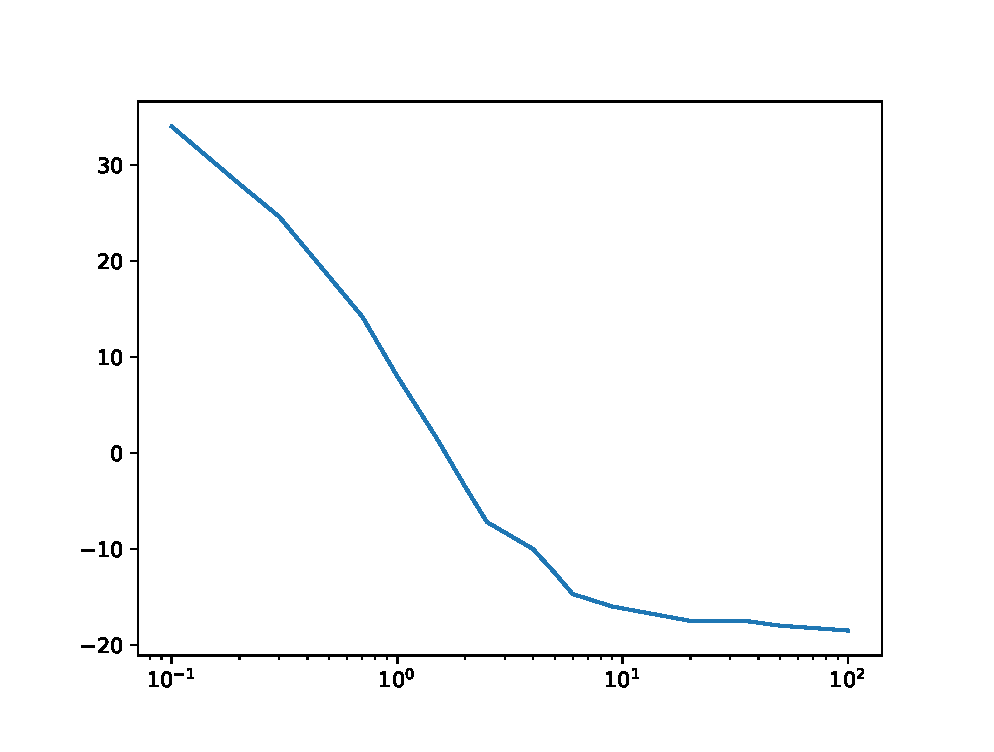
\includegraphics[width=\columnwidth]{./figs/ee18btech11006/ee18btech11006_1.eps}
\caption{1}
\label{fig:ee18btech11006_1}
\end{figure}
Consider the Transfer function
\begin{align}
H(s) &= \frac{k\brak{s+z_{1}}\brak{s+z_{2}}}{\brak{s+p_{1}}\brak{s+p_{2}}} 
\end{align}
Let's draw the magnitude bode plot.
\\
\solution 
\begin{enumerate}

\begin{multline}
20log_{10}|H(s)| = 20log_{10}|s+z_{1}|+20log_{10}|s+z_{2}|\\
-20log_{10}|s+p_{1}|-20log_{10}|s+p_{2}|\\
+20log_{10}k
\end{multline}

For every zero the slope of the magnitude curve increases by 20dB/dec and for every pole it decreases by 20dB/dec.\\
Now, for the given set of points finding slopes corresponding to every two points and identifying the points at which the slope change occurs would give us the poles and zeros respectively.\\
The slope initially is-20dB/decade i.e. pole at 0.1 \\
We can observe that the slope decreases approximately by 20dB/dec at the point 0.7 and increases further by 20dB/dec at 2.5 and 6 giving a slope of almost 0 later on. 
\begin{align}
Poles&= 0.1,0.7\\
Zeros&= 2.5,6
\end{align}
Lets plot the magnitude bode plot considering these poles and zeros.\\
The following code generates the plot for the transfer function
\begin{align}
H(s) &= \frac{\brak{s+2.5}\brak{s+6}}{\brak{s+0.1}\brak{s+0.7}}
\end{align}
\begin{lstlisting}
codes/ee18btech11006/ee18btech11006_2.py
\end{lstlisting}
\begin{figure}[!ht]
\centering
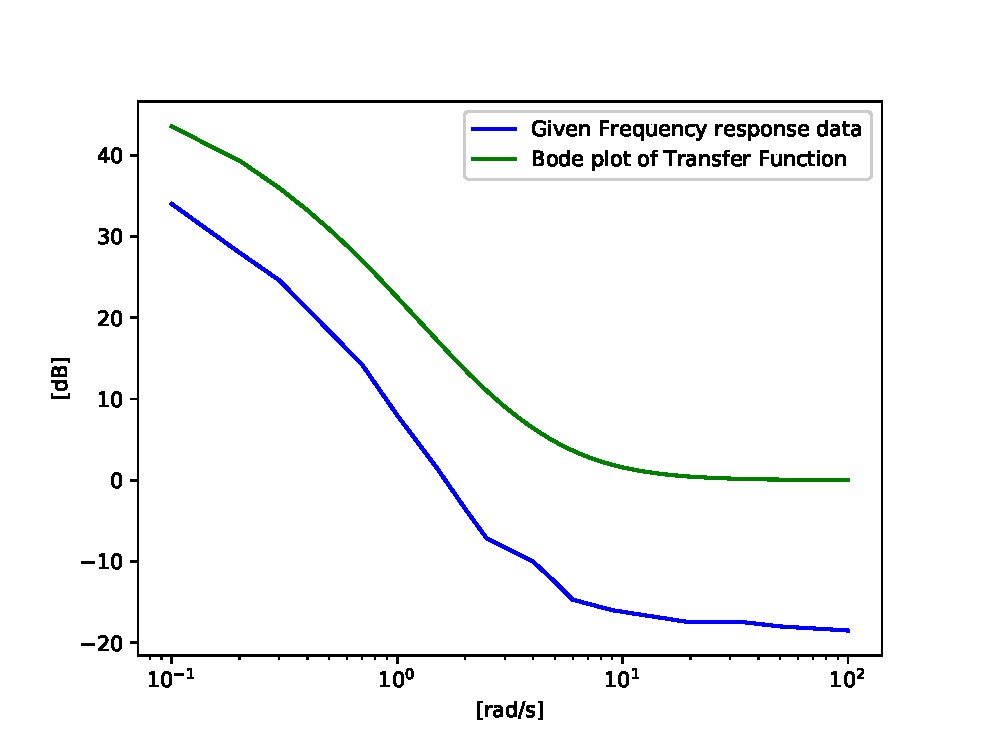
\includegraphics[width=\columnwidth]{./figs/ee18btech11006/ee18btech11006_2.eps}
\caption{2}
\label{fig:ee18btech11006_2}
\end{figure}
Now the gain,
\begin{align}
K=\frac{H\brak{w}\brak{given}}{H\brak{w}\brak{calculated}} 
\end{align}
This value would vary for different values of w.\\
Considering the average value , K= 0.1778. \\
The following code generates the plot for the transfer function
\begin{align}
H(s) &= \frac{0.1778\brak{s+2.5}\brak{s+6}}{\brak{s+0.1}\brak{s+0.7}} 
\end{align}
\begin{lstlisting}
codes/ee18btech11006/ee18btech11006_3.py
\end{lstlisting}
\begin{figure}[!ht]
\centering
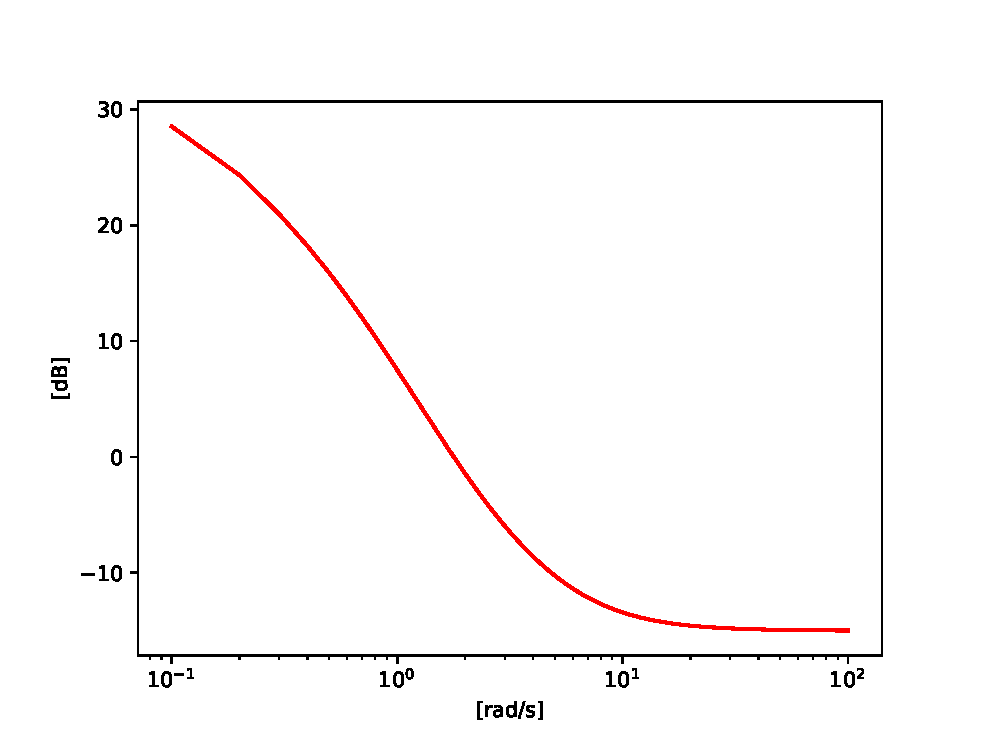
\includegraphics[width=\columnwidth]{./figs/ee18btech11006/ee18btech11006_3.eps}
\caption{3}
\label{fig:ee18btech11006_3}
\end{figure}
Thus, our Transfer function is 
\begin{align}
H(s) &= \frac{0.1778\brak{s+2.5}\brak{s+6}}{\brak{s+0.1}\brak{s+0.7}}  
\end{align}
\end{enumerate}

\caption{}
\label{table:ee18btech11006}
\end{table}\\
\solution 
The following code generates the plot for the given data.
\begin{lstlisting}
codes/ee18btech11006/ee18btech11006_1.py
\end{lstlisting}
\begin{figure}[!ht]
\centering
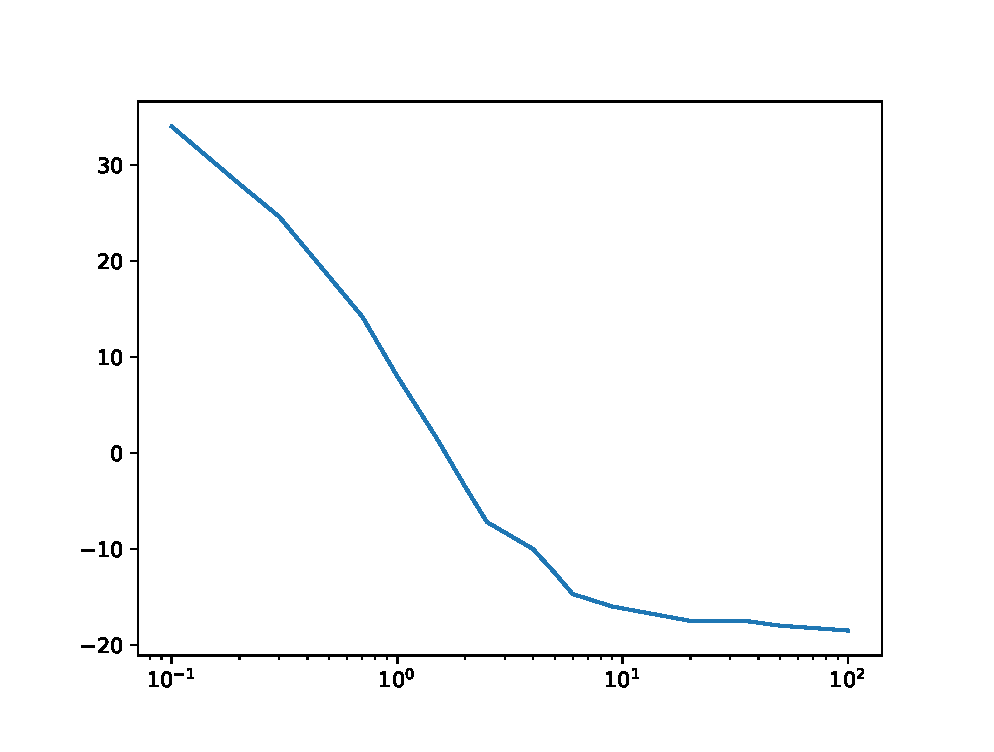
\includegraphics[width=\columnwidth]{./figs/ee18btech11006/ee18btech11006_1.eps}
\caption{1}
\label{fig:ee18btech11006_1}
\end{figure}
Consider the Transfer function
\begin{align}
H(s) &= \frac{k\brak{s+z_{1}}\brak{s+z_{2}}}{\brak{s+p_{1}}\brak{s+p_{2}}} 
\end{align}
Let's draw the magnitude bode plot.
\\
\solution 
\begin{enumerate}

\begin{multline}
20log_{10}|H(s)| = 20log_{10}|s+z_{1}|+20log_{10}|s+z_{2}|\\
-20log_{10}|s+p_{1}|-20log_{10}|s+p_{2}|\\
+20log_{10}k
\end{multline}

For every zero the slope of the magnitude curve increases by 20dB/dec and for every pole it decreases by 20dB/dec.\\
Now, for the given set of points finding slopes corresponding to every two points and identifying the points at which the slope change occurs would give us the poles and zeros respectively.\\
The slope initially is-20dB/decade i.e. pole at 0.1 \\
We can observe that the slope decreases approximately by 20dB/dec at the point 0.7 and increases further by 20dB/dec at 2.5 and 6 giving a slope of almost 0 later on. 
\begin{align}
Poles&= 0.1,0.7\\
Zeros&= 2.5,6
\end{align}
Lets plot the magnitude bode plot considering these poles and zeros.\\
The following code generates the plot for the transfer function
\begin{align}
H(s) &= \frac{\brak{s+2.5}\brak{s+6}}{\brak{s+0.1}\brak{s+0.7}}
\end{align}
\begin{lstlisting}
codes/ee18btech11006/ee18btech11006_2.py
\end{lstlisting}
\begin{figure}[!ht]
\centering
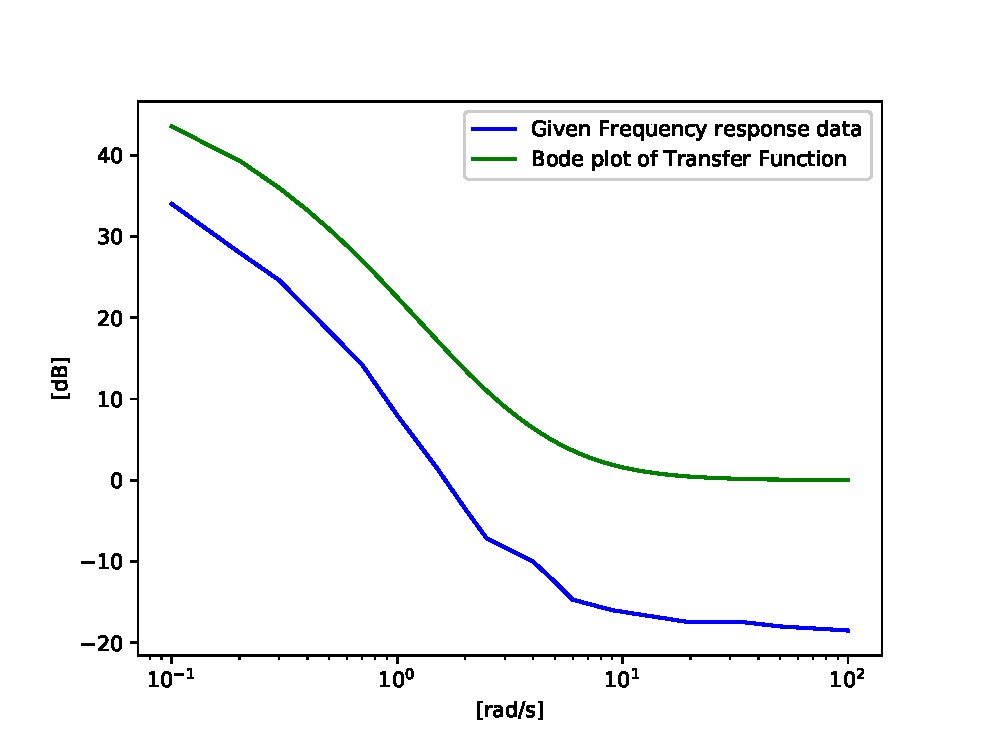
\includegraphics[width=\columnwidth]{./figs/ee18btech11006/ee18btech11006_2.eps}
\caption{2}
\label{fig:ee18btech11006_2}
\end{figure}
Now the gain,
\begin{align}
K=\frac{H\brak{w}\brak{given}}{H\brak{w}\brak{calculated}} 
\end{align}
This value would vary for different values of w.\\
Considering the average value , K= 0.1778. \\
The following code generates the plot for the transfer function
\begin{align}
H(s) &= \frac{0.1778\brak{s+2.5}\brak{s+6}}{\brak{s+0.1}\brak{s+0.7}} 
\end{align}
\begin{lstlisting}
codes/ee18btech11006/ee18btech11006_3.py
\end{lstlisting}
\begin{figure}[!ht]
\centering
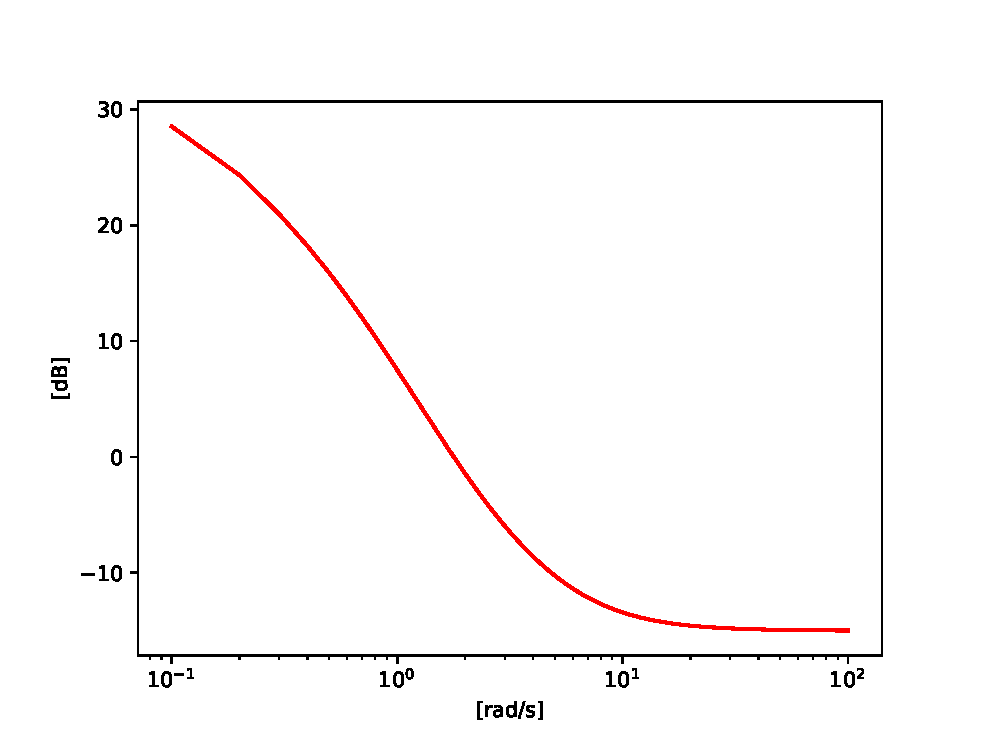
\includegraphics[width=\columnwidth]{./figs/ee18btech11006/ee18btech11006_3.eps}
\caption{3}
\label{fig:ee18btech11006_3}
\end{figure}
Thus, our Transfer function is 
\begin{align}
H(s) &= \frac{0.1778\brak{s+2.5}\brak{s+6}}{\brak{s+0.1}\brak{s+0.7}}  
\end{align}
\end{enumerate}

\caption{}
\label{table:ee18btech11006}
\end{table}\\
\solution 
The following code generates the plot for the given data.
\begin{lstlisting}
codes/ee18btech11006/ee18btech11006_1.py
\end{lstlisting}
\begin{figure}[!ht]
\centering
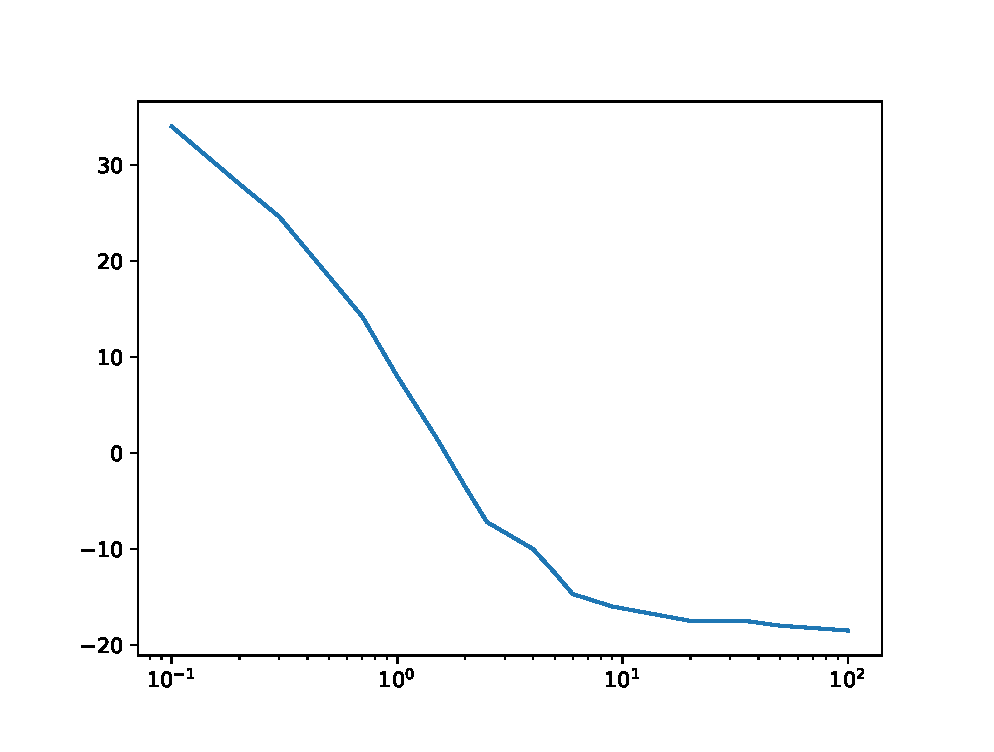
\includegraphics[width=\columnwidth]{./figs/ee18btech11006/ee18btech11006_1.eps}
\caption{1}
\label{fig:ee18btech11006_1}
\end{figure}
Consider the Transfer function
\begin{align}
H(s) &= \frac{k\brak{s+z_{1}}\brak{s+z_{2}}}{\brak{s+p_{1}}\brak{s+p_{2}}} 
\end{align}
Let's draw the magnitude bode plot.
\\
\solution 
\begin{enumerate}

\begin{multline}
20log_{10}|H(s)| = 20log_{10}|s+z_{1}|+20log_{10}|s+z_{2}|\\
-20log_{10}|s+p_{1}|-20log_{10}|s+p_{2}|\\
+20log_{10}k
\end{multline}

For every zero the slope of the magnitude curve increases by 20dB/dec and for every pole it decreases by 20dB/dec.\\
Now, for the given set of points finding slopes corresponding to every two points and identifying the points at which the slope change occurs would give us the poles and zeros respectively.\\
The slope initially is-20dB/decade i.e. pole at 0.1 \\
We can observe that the slope decreases approximately by 20dB/dec at the point 0.7 and increases further by 20dB/dec at 2.5 and 6 giving a slope of almost 0 later on. 
\begin{align}
Poles&= 0.1,0.7\\
Zeros&= 2.5,6
\end{align}
Lets plot the magnitude bode plot considering these poles and zeros.\\
The following code generates the plot for the transfer function
\begin{align}
H(s) &= \frac{\brak{s+2.5}\brak{s+6}}{\brak{s+0.1}\brak{s+0.7}}
\end{align}
\begin{lstlisting}
codes/ee18btech11006/ee18btech11006_2.py
\end{lstlisting}
\begin{figure}[!ht]
\centering
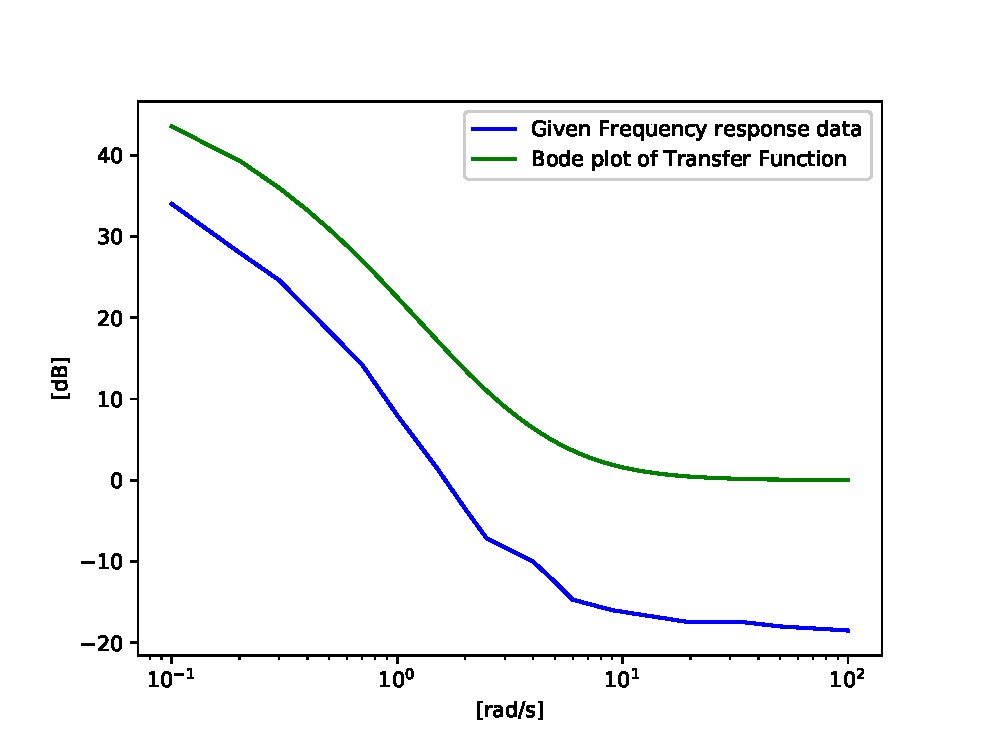
\includegraphics[width=\columnwidth]{./figs/ee18btech11006/ee18btech11006_2.eps}
\caption{2}
\label{fig:ee18btech11006_2}
\end{figure}
Now the gain,
\begin{align}
K=\frac{H\brak{w}\brak{given}}{H\brak{w}\brak{calculated}} 
\end{align}
This value would vary for different values of w.\\
Considering the average value , K= 0.1778. \\
The following code generates the plot for the transfer function
\begin{align}
H(s) &= \frac{0.1778\brak{s+2.5}\brak{s+6}}{\brak{s+0.1}\brak{s+0.7}} 
\end{align}
\begin{lstlisting}
codes/ee18btech11006/ee18btech11006_3.py
\end{lstlisting}
\begin{figure}[!ht]
\centering
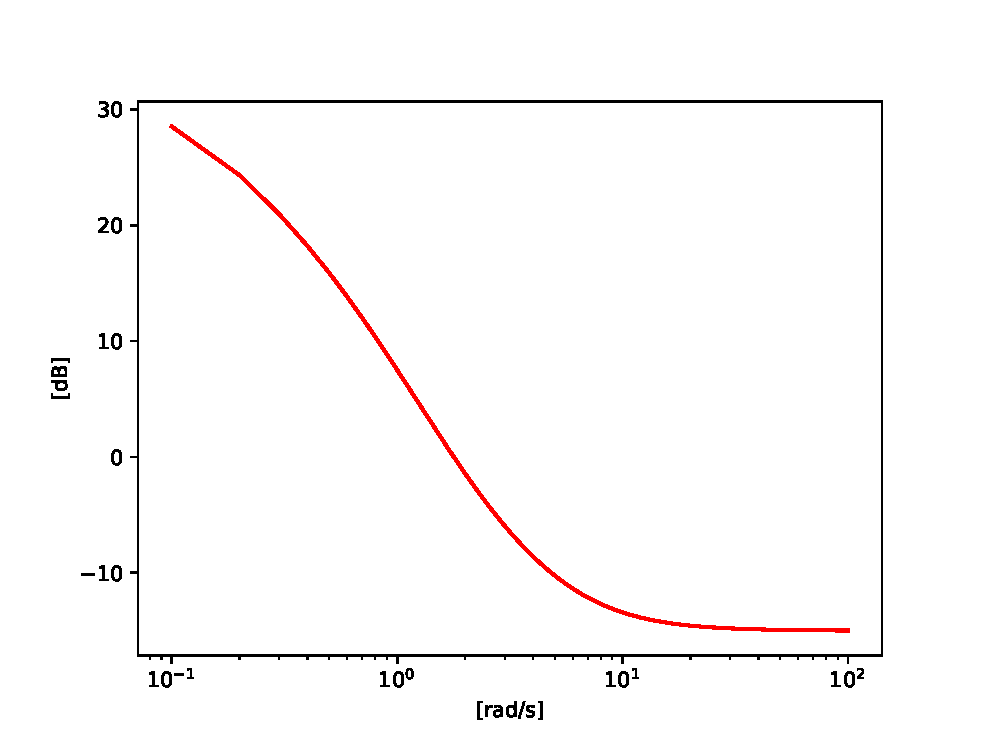
\includegraphics[width=\columnwidth]{./figs/ee18btech11006/ee18btech11006_3.eps}
\caption{3}
\label{fig:ee18btech11006_3}
\end{figure}
Thus, our Transfer function is 
\begin{align}
H(s) &= \frac{0.1778\brak{s+2.5}\brak{s+6}}{\brak{s+0.1}\brak{s+0.7}}  
\end{align}
\end{enumerate}

\caption{}
\label{table:ee18btech11006}
\end{table}\\
\solution 
The following code generates the plot for the given data.
\begin{lstlisting}
codes/ee18btech11006/ee18btech11006_1.py
\end{lstlisting}
\begin{figure}[!ht]
\centering
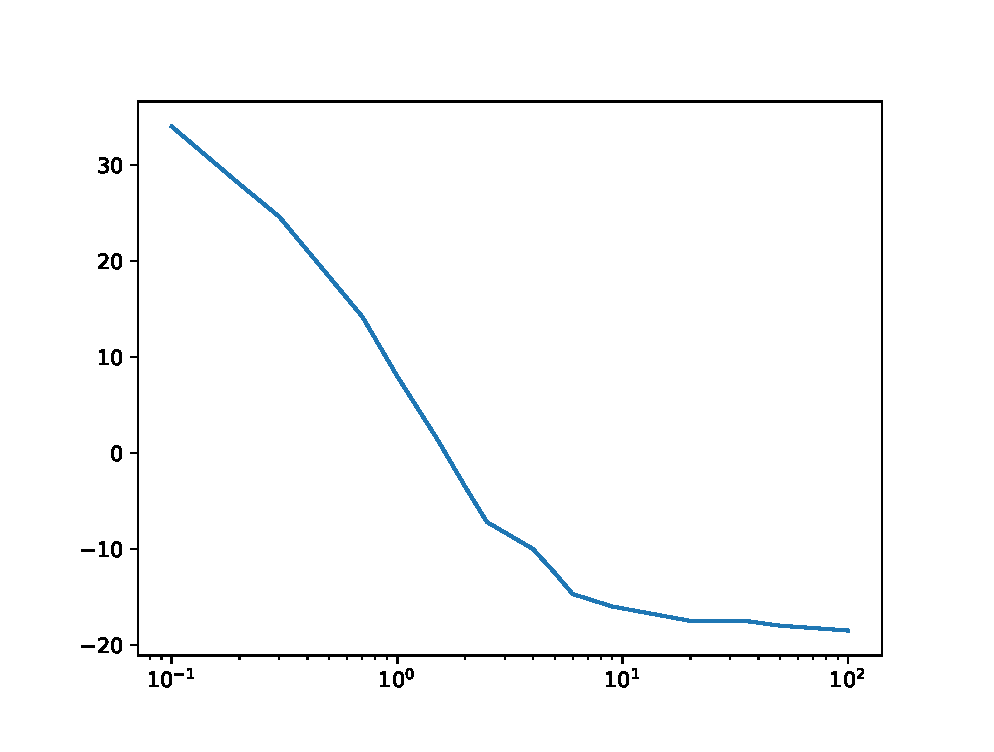
\includegraphics[width=\columnwidth]{./figs/ee18btech11006/ee18btech11006_1.eps}
\caption{1}
\label{fig:ee18btech11006_1}
\end{figure}
Consider the Transfer function
\begin{align}
H(s) &= \frac{k\brak{s+z_{1}}\brak{s+z_{2}}}{\brak{s+p_{1}}\brak{s+p_{2}}} 
\end{align}
Let's draw the magnitude bode plot.
\\
\solution 
\begin{enumerate}

\begin{multline}
20log_{10}|H(s)| = 20log_{10}|s+z_{1}|+20log_{10}|s+z_{2}|\\
-20log_{10}|s+p_{1}|-20log_{10}|s+p_{2}|\\
+20log_{10}k
\end{multline}

For every zero the slope of the magnitude curve increases by 20dB/dec and for every pole it decreases by 20dB/dec.\\
Now, for the given set of points finding slopes corresponding to every two points and identifying the points at which the slope change occurs would give us the poles and zeros respectively.\\
The slope initially is-20dB/decade i.e. pole at 0.1 \\
We can observe that the slope decreases approximately by 20dB/dec at the point 0.7 and increases further by 20dB/dec at 2.5 and 6 giving a slope of almost 0 later on. 
\begin{align}
Poles&= 0.1,0.7\\
Zeros&= 2.5,6
\end{align}
Lets plot the magnitude bode plot considering these poles and zeros.\\
The following code generates the plot for the transfer function
\begin{align}
H(s) &= \frac{\brak{s+2.5}\brak{s+6}}{\brak{s+0.1}\brak{s+0.7}}
\end{align}
\begin{lstlisting}
codes/ee18btech11006/ee18btech11006_2.py
\end{lstlisting}
\begin{figure}[!ht]
\centering
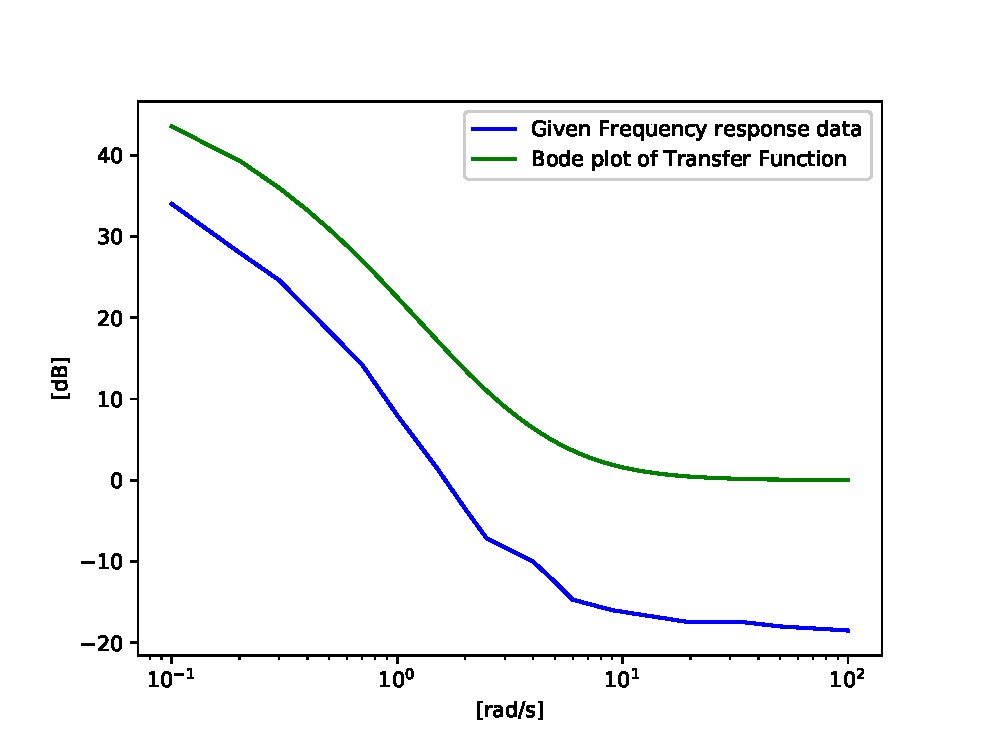
\includegraphics[width=\columnwidth]{./figs/ee18btech11006/ee18btech11006_2.eps}
\caption{2}
\label{fig:ee18btech11006_2}
\end{figure}
Now the gain,
\begin{align}
K=\frac{H\brak{w}\brak{given}}{H\brak{w}\brak{calculated}} 
\end{align}
This value would vary for different values of w.\\
Considering the average value , K= 0.1778. \\
The following code generates the plot for the transfer function
\begin{align}
H(s) &= \frac{0.1778\brak{s+2.5}\brak{s+6}}{\brak{s+0.1}\brak{s+0.7}} 
\end{align}
\begin{lstlisting}
codes/ee18btech11006/ee18btech11006_3.py
\end{lstlisting}
\begin{figure}[!ht]
\centering
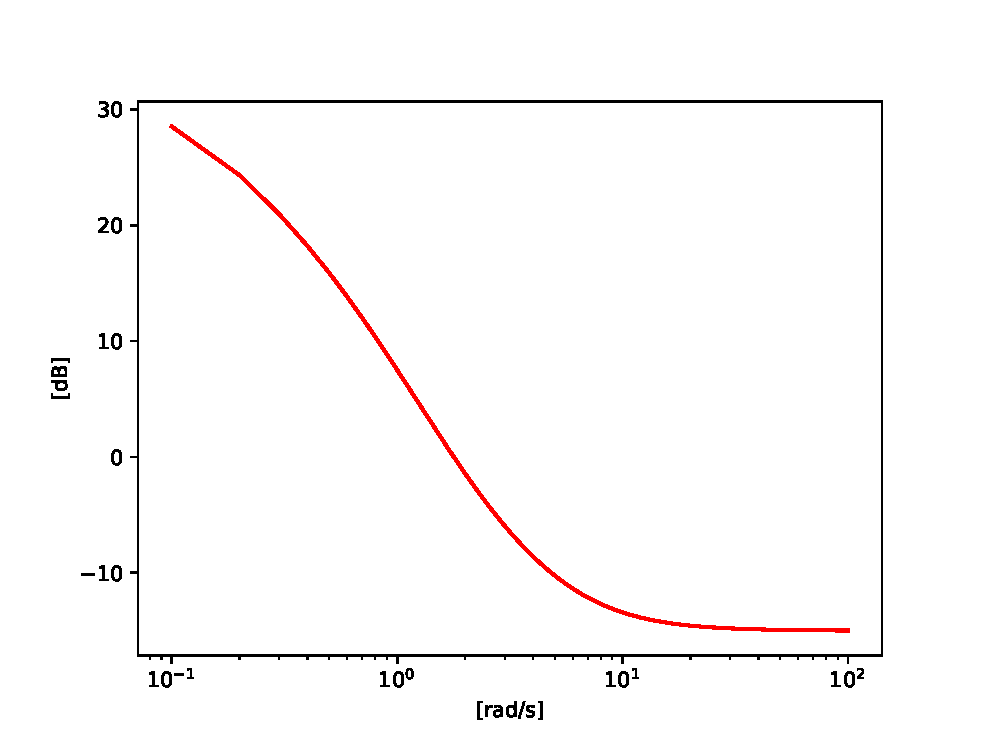
\includegraphics[width=\columnwidth]{./figs/ee18btech11006/ee18btech11006_3.eps}
\caption{3}
\label{fig:ee18btech11006_3}
\end{figure}
Thus, our Transfer function is 
\begin{align}
H(s) &= \frac{0.1778\brak{s+2.5}\brak{s+6}}{\brak{s+0.1}\brak{s+0.7}}  
\end{align}
\end{enumerate}
